\chapter{Implementation Details}

\section{Document management}

The current section consists of three parts:

\begin{itemize}
\item The first one explains the prototype we wrote.
\item The second one details implementation challenges when realizing the designed extension and using external libraries.
\item The third one shows changes in the extension visible from a user's point of view, with screenshots.
\end{itemize}

\subsection{The prototype}

As mentioned already, the SharePoint protocol has a brief reference
documentation on MSDN, but that is not enough to create an open-source
implementation of the protocol. To solve that issue, we used two virtual
machines:

\begin{itemize}
\item One running Microsoft SharePoint 2007.
\item The other running Microsoft Office 2007.
\end{itemize}

Finally, we used Wireshark \cite{wireshark} to monitor the network traffic
between the two virtual machines to reverse engineer the details of the
protocol missing from the reference documentation.

Trying to reimplement the protocol directly in the LibreOffice extension would
make development slow, partly because that would mean solving UNO interfacing
issues and Java design decisions at the same time, partly because we needed a
simple script to demonstrate how the protocol works, where Java may not be the
best language to use. As a consequence, we decided to write a command-line
prototype in Python, a popular scripting language, and once that was ready and
worked, we ported the logic of the prototype to Java.

The prototype had commands (open, save, delete, etc.) to test each feature
individually.  This covered the functionality outlined in the \emph{Background}
chapter, except that folder / document listing is implicit here: the open and
save-as operation invoked that, but it had no explicit command assigned.

The prototype also had two switches to test the implementation on both
SharePoint and Alfresco automatically. This was critical, so that when we fixed
something to work with Alfresco, we could quickly test that we did not break
anything in SharePoint.

\subsection{The SharePoint protocol}

This subsection gives a brief overview of the SharePoint protocol; for the
exact details, see the source code of our solution. Note that this analysis may
not be fully accurate, it is only the understanding of the author, and was good
enough to serve as a base of the implementation.

Definitions:

\begin{itemize}
\item workspace: a top-level directory, contains folders
\item folder: a non-top-level directory, contains folders and documents
\item document: several versions of the same file, identified by version numbers
\item checkout, checkin, uncheckout: acquiring and releasing a lock on the document
\end{itemize}

The following workspace management operations are supported by the SharePoint
library:

\begin{enumerate}
\item login: simply tries to access \texttt{/\_vti\_inf.html} on the server with the provided credentials

\item create workspace: SOAP request to \texttt{/\_vti\_bin/dws.asmx} in the site root
\begin{itemize}
\item method name: \texttt{CreateDws}
\item parameters: \texttt{title} (name of the workspace)
\item returns: the HTTP status code (200 means success) can be used to check if the operation was successful
\end{itemize}

\item list workspaces: RPC request to \texttt{/\_vti\_bin/\_vti\_aut/author.dll} in the site root
\begin{itemize}
\item method name: \texttt{list documents}
\item parameters: none
\item returns: HTML page, a single enumeration provides the URL of the workspaces
\end{itemize}

\item delete workspace: SOAP request to \texttt{/\_vti\_bin/dws.asmx} in the workspace root
\begin{itemize}
\item method name: \texttt{DeleteDws}
\item parameters: none
\item returns: the HTTP status code (200 means success) can be used to check if the operation was successful
\end{itemize}
\end{enumerate}

Folder management:

\begin{enumerate}
\item create folder: SOAP request to \texttt{/\_vti\_bin/dws.asmx} in the site root
\begin{itemize}
\item method name: \texttt{CreateFolder}
\item parameters: \texttt{url} (url of the folder)
\item returns: the HTTP status code (200 means success) can be used to check if the operation was successful
\end{itemize}

\item list folders: HTTP GET to \texttt{/\_vti\_bin/owssvr.dll} in the workspace root
\begin{itemize}
\item parameters: \texttt{location} (URL of the folder), \texttt{FileDialogFilterValue} (filter to apply to the result on server side, for example \texttt{*.*})
\item returns: HTML page, containing a table where every row is a folder or a
document and each column contains properties of the item. The property names
can be configured in runtime on the server.
\end{itemize}

\item delete folder: SOAP request to \texttt{/\_vti\_bin/dws.asmx} in the site root
\begin{itemize}
\item method name: \texttt{DeleteDws}
\item parameters: \texttt{url} (url of the folder)
\item returns: the HTTP status code (200 means success) can be used to check if the operation was successful
\end{itemize}
\end{enumerate}

Document management:

\begin{enumerate}
\item open: no dedicated method, HTTP GET should be used with the URL's returned by \emph{list folders}
\item save: RPC request to \texttt{/\_vti\_bin/\_vti\_aut/author.dll} in the workspace root
\begin{itemize}
\item method name: \texttt{put document} (yes, RPC method names can contain spaces)
\item parameters: \texttt{service\_name} (name of the workspace), \texttt{document} (structure containing the document name and last modification date), \texttt{comment} (this option should be provided, but its value is ignored)
\item payload: everything after two newline characters is considered as the document data
\item returns: an RPC response packet, containing a "successfully put document" string with a \texttt{msg=} or \texttt{message=} prefix
\end{itemize}

\item remove documents: RPC request to \texttt{/\_vti\_bin/\_vti\_aut/author.dll} in the workspace root
\begin{itemize}
\item method name: \texttt{remove documents}
\item parameters: \texttt{url\_list} (list of URL's to remove)
\item returns: an RPC response packet, containing a "successfully put document" string with a \texttt{msg=} or \texttt{message=} prefix
\end{itemize}

\item get document metadata: RPC request to \texttt{/\_vti\_bin/\_vti\_aut/author.dll} in the workspace root
\begin{itemize}
\item method name: \texttt{getDocsMetaInfo}
\item parameters: \texttt{url\_list} (list of URL's to query)
\item returns: several HTML enumerations, one for each URL
\end{itemize}
\end{enumerate}

Lock management:

\begin{enumerate}
\item checkout: SOAP request to \texttt{/\_vti\_bin/lists.asmx} in the workspace root
\begin{itemize}
\item method name: \texttt{CheckOutFile}
\item parameters: \texttt{pageUrl} (URL of the document to check out), \texttt{lastmodified} (last modification date of the document, in case the document is already opened but not checked out)
\item returns: \texttt{CheckOutFileResult}, containing a boolean value
\end{itemize}

\item checkin: SOAP request to \texttt{/\_vti\_bin/lists.asmx} in the workspace root
\begin{itemize}
\item method name: \texttt{CheckInFile}
\item parameters: \texttt{pageUrl} (URL of the document to check in), \texttt{comment} (the "commit message") and \texttt{CheckinType} (0 = \texttt{MinorCheckIn}, 1 = \texttt{MajorCheckIn}, and 2 = \texttt{OverwriteCheckIn})
\item returns: \texttt{CheckInFileResult}, containing a boolean value
\end{itemize}

\item undo checkout: SOAP request to \texttt{/\_vti\_bin/lists.asmx} in the workspace root
\begin{itemize}
\item method name: \texttt{UndoCheckOut}
\item parameters: \texttt{pageUrl} (URL of the document to uncheckout)
\item returns: \texttt{UndoCheckOutResponse}, containing a boolean value
\end{itemize}
\end{enumerate}

Version management:

\begin{enumerate}
\item create version: no dedicated method, a \emph{save} or \emph{checkin} can create a new version
\item list versions: SOAP request to \texttt{/\_vti\_bin/versions.asmx} in the workspace root
\begin{itemize}
\item method name: \texttt{GetVersions}
\item parameters: \texttt{fileName} (URL of the document)
\item returns: a list of \texttt{result} elements -- each contains "version", "created", "createdBy", "size", "comments" and "url" fields
\end{itemize}

\item restore version: SOAP request to \texttt{/\_vti\_bin/versions.asmx} in the workspace root
\begin{itemize}
\item method name: \texttt{RestoreVersion}
\item parameters: \texttt{fileName} (URL of the document to restore), \texttt{fileVersion} (old version number)
\item returns: a list of \texttt{soap:Fault} elements -- if it is empty, it means success
\end{itemize}

\item delete version: SOAP request to \texttt{/\_vti\_bin/versions.asmx} in the workspace root
\begin{itemize}
\item method name: \texttt{DeleteVersion}
\item parameters: \texttt{fileName} (URL of the document), \texttt{fileVersion} (version number)
\item returns: a list of \texttt{soap:Fault} elements -- if it is empty, it means success
\end{itemize}

\end{enumerate}

In all SOAP requests an additional \texttt{X-Office-Version} header is
necessary, the value of this header is 12.0.6514 for Office 2007.

In RPC requests, the two following headers are necessary:

\begin{lstlisting}
Content-Type: application/x-vermeer-urlencoded
X-Vermeer-Content-Type: application/x-vermeer-urlencoded
\end{lstlisting}

Once the details of the protocol -- at least the parts required for our use-cases -- were
clear, we could begin writing the LibreOffice extension.

\subsection{External libraries}

It was obvious that doing HTTP communication with NTLM authentication is an
already solved problem, but we needed to decide which library to use. Given that
OPAL already used Apache \emph{commons-httpclient} \cite{httpclient} 3.x for
HTTP communication, that was an option. Unfortunately that version does not support NTLM, so we used
Apache \emph{httpcomponents} \cite{httpcomponents}, which is the successor of
the previous library (starting with version 4.x). The two version series have
different APIs, so it was possible to temporarily use both in parallel, and migrating code
incrementally.

Once we had \emph{httpcomponents}, we still needed to write detection code that
decided what to request from \emph{httpcomponents}: Basic or NTLM
authentication.

An other interesting issue was to parse the response received after sending
Vermeer RPC requests to the server. The result is valid HTML, but not XHTML.
For example, part of the response is:

\begin{lstlisting}
<html><head><title>vermeer RPC packet</title></head>
<body>
...
<li>vti_timecreated
<li>TR|27 Feb 2011 19:07:25 +0000
<li>vti_timelastmodified
<li>TR|11 Mar 2011 16:39:35 +0000
<li>vti_timelastwritten
<li>TR|11 Mar 2011 16:39:35 +0000
...
</body>
</html>\end{lstlisting}

That means a simple XML parser was not enough to extract the needed values from
this response. To solve this issue, we used TagSoup \cite{tagsoup}, which is a
SAX parser, accepting plain old HTML input.

\subsection{User interface}

Once the Sharpeoint Library was ready, we updated the user interface to use the
SharePoint library for communication. We also had to extend the dialogs to allow
a few more features. Namely:

\begin{itemize}
\item Create and delete document workspaces.
\item Delete documents.
\item Delete and restore versions.
\item When saving a document, allow: minor change with a comment and overwrite of a previous version.
\end{itemize}

For example, creating a new document workspace is implemented as can be seen on
\autoref{fig:implementation-createdws}.

\begin{figure}[H]
\centering
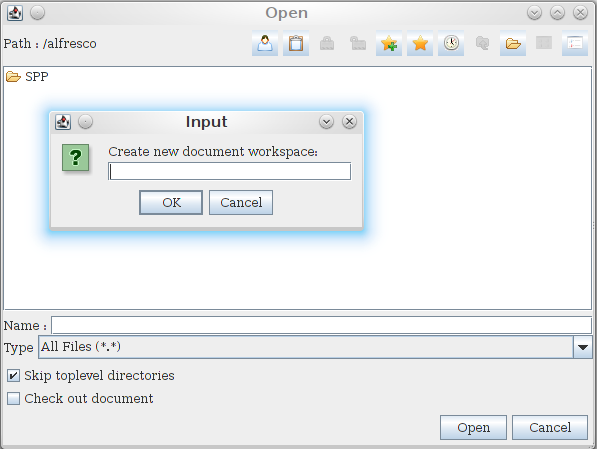
\includegraphics[width=250px,keepaspectratio]{implementation-createdws.png}
\caption{Implementation of creating a document workspace}
\label{fig:implementation-createdws}
\end{figure}

Earlier only viewing older versions was possible; the new \emph{Versions}
dialog now allows a user to delete and restore versions as well (as detailed
above in \autoref{tab:background-comparison}, deleting versions does not work
with Alfresco, due to the shortcomings of their SharePoint implementation), see
\autoref{fig:implementation-versiondialog}.

\begin{figure}[H]
\centering
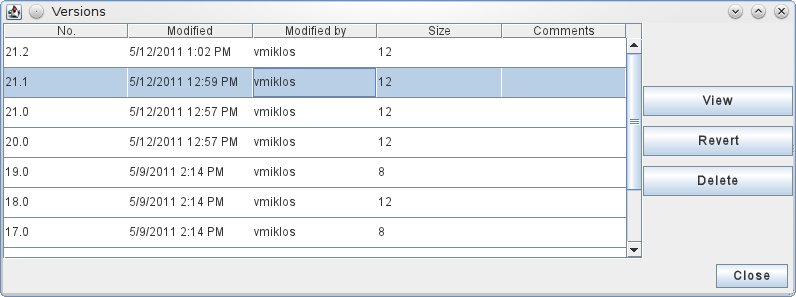
\includegraphics[width=300px,keepaspectratio]{implementation-versiondialog.png}
\caption{Implementation of version restore and delete}
\label{fig:implementation-versiondialog}
\end{figure}

\subsection{Exception handling}

The last challenge was the localization of error messages in BASIC. The
language does not support any kind of localization. What it supports is the
following technique (control flow shown on \autoref{fig:basic-l10n}):

\begin{lstlisting}
Sub openVersion
...
        On Error GoTo errSpDoc
        oVersion.execute()
        Exit Sub

        errSpDoc:
                MsgBox(oVersion.ErrorReason)
                Exit Sub
End Sub
\end{lstlisting}

\begin{figure}[H]
\centering
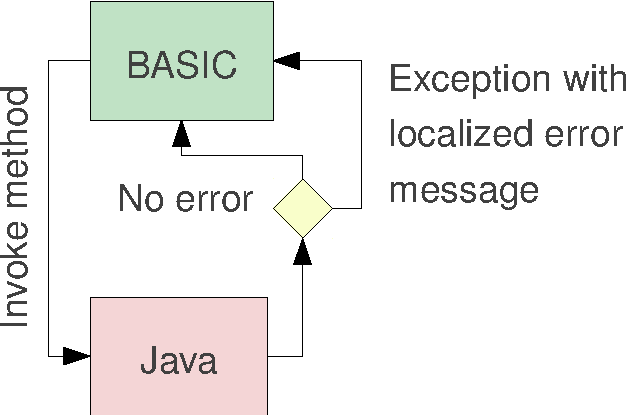
\includegraphics[width=200px,keepaspectratio]{basic-l10n.pdf}
\caption{Control flow of localized error messages in BASIC, thrown by Java.}
\label{fig:basic-l10n}
\end{figure}

The \emph{On Error} part can hide any kind of exception thrown by Java, and as
long as the Java side calls \emph{setErrorReason()} on the
\emph{SharepointVersionsImpl} object before throwing an exception, the user gets
a friendly error message, which is even localized.

\section{Workflows}

The implementation of workflow integration had multiple interesting challenges:

\begin{itemize}
\item adding support for the authentication method jBPM uses
\item handling data received in responses from jBPM
\item error handling in multiple levels
\end{itemize}

\subsection{Authentication}

The jBPM uses form-based authentication. That means that in case the user is not
yet logged in, he/she is redirected to a login form, where the user name and
password should be submitted. The \emph{httpcomponents} package provides a
dedicated \emph{UrlEncodedFormEntity} class for this purpose:

\begin{itemize}
\item Fields in the form should be collected in a \emph{NameValuePair} list;
\item Once the list is ready, the entity generator class can produce the
necessary payload for the HTTP request, using the
\texttt{application/x-www-form-urlencoded} MIME type \cite{form-encoding}.
\end{itemize}

There are two problems here:

\begin{itemize}
\item The user interface expects a stateful connection here, while HTTP is stateless.
\item The password is sent without encryption.
\end{itemize}

The first problem can be solved multiple ways. First, the workflow handler can
remember the credentials passed from the user interface, hiding the repeated
login procedure from the user. Alternatively, in this case jBPM handles
sessions, so receiving and sending back cookies avoids multiple logins as well.

The problem of clear-text passwords sent over the network can be solved at an
application server level, in case HTTPS is used.

From a user experience point of view an additional problem is the confusing
connection dialog that asks for multiple user names and passwords. Given that
we are integrating the document management and the workflow system, we can
expect that the same credentials are used by the same users to access these
servers. As a result, the user interface asks for a single login and password,
the Java implementation does two logins in practice, though. The user interface
signals an error in case any of these logins failed.

\subsection{JSON handling}

Most responses received from the jBPM server are JavaScript Object Notation
(JSON) strings. The interested reader can look into the
specification \cite{json}, all we need to know about it here is that it can
represent a set of Java objects, allowing references between them.

Once entity classes are available (as described in the \emph{Design} chapter),
the Gson library \cite{gson} can be used to parse those strings to entity class
instances.

The benefits of using Gson over other implementations (like
\emph{org.json} \cite{org-json}):

\begin{itemize}
\item it requires no pollution of the entity classes regarding JSON (i.e. no \emph{toJson()} methods are necessary)
\item when a default constructor is not available for an entity class, it supports the registration of instance creators for such types
\end{itemize}

It uses reflection to access fields, so the general object-oriented methodology
where the fields themselves are private and public getter/setter methods are
provided is possible to use. Also, the parser is quite liberal about entity
classes, in case a field is present in the JSON string but the associated Java
class does not have such a field, it is simply ignored. That helps our
extension to be compatible with future jBPM server versions.

A pitfall during the implementation was that the usage of generic types is
mandatory when using references between the classes:

\begin{itemize}
\item In case a generalized collection is used as a field type, Gson can extract the type information of the referenced objects from the field type, and instantiate the correct class.
\item Otherwise, there is no way to guess the type of the referenced instance, so a parse exception is thrown.
\end{itemize}

\subsection{User interface}

\notocsubsubsection{Private streams}

The first challenge was to map the concepts of a user and the associated
personal / group tasks to the file / folder metaphor, already known by users.

In LibreOffice, access to files is usually handled by a sequence of property
values (key-value pairs), where usually the \emph{URL} property is used to
access the physical file. However in some cases there is no real URL, but the
contents of the object are provided as a \emph{Stream} property.  An example is
the framework module \cite{lo-framework-module}, where even a define (with a
value of \emph{private:stream}) is provided to be used as a fake URL for such
streams.  A similar constant is available to access factories with a
\emph{private:factory} URL. Using that URL e.g. in Writer, a new empty document
is opened.

Extending this technique, the extension introduces the following identifiers in
the \emph{private:} namespace:

\begin{itemize}
\item \emph{private:personaltasks} is used to access personal tasks
\item \emph{private:grouptasks} is used to access group tasks
\end{itemize}

The \emph{WFHandler.urlopen()} method, which was originally designed to open
regular URL's, can handle these special ones. During the opening operation it performs the following steps:

\begin{itemize}
\item It queries task instances of the given task type from the workflow server.
\item Once a task instance is selected, it extracts the associated document URL from the associated process instance variables.
\item Finally, the extension already knows how to open a document server URL.
\end{itemize}

\begin{figure}[H]
\centering
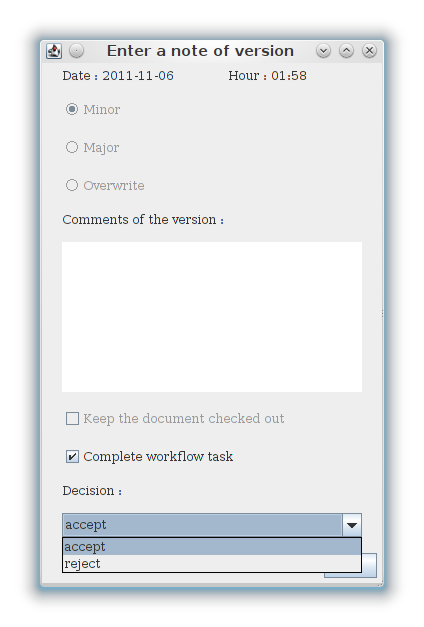
\includegraphics[width=200px,keepaspectratio]{implementation-decision.png}
\caption{Implementation of making a business decision when completing a human task}
\label{fig:implementation-decision}
\end{figure}

During save, the \emph{CommentVersionDialog} class invokes \emph{WFHandler} to
check if the document has a task associated. If so, the two controls at the
bottom of the dialog are enabled to control the interaction with the workflow
server during save (see \autoref{fig:implementation-decision}):

\begin{itemize}
\item if the workflow should be stepped
\item the answer to the business decision, if available
\end{itemize}

\notocsubsubsection{Audit log}

The second new menu item introduced by the workflow integration is the audit
log. First a dialog asks the process type to audit (similar to the process
definition selector when starting a new process instance), then the list of
historic process instances appear.

\begin{figure}[H]
\centering
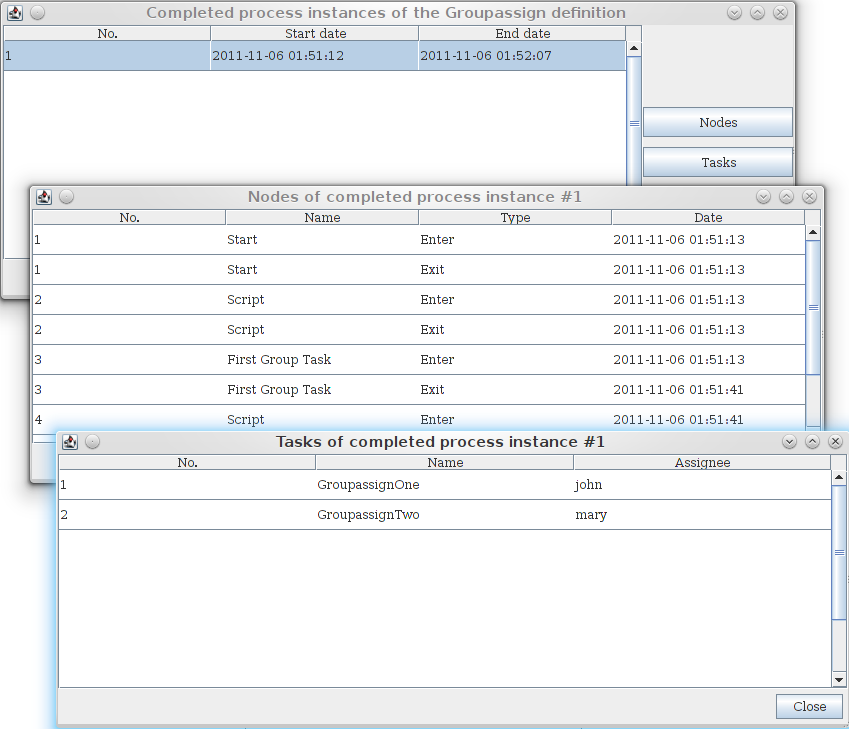
\includegraphics[width=400px,keepaspectratio]{implementation-auditlog.png}
\caption{Implementation of the audit log: process instances, node instances and users performing human tasks}
\label{fig:implementation-auditlog}
\end{figure}

Buttons next to this table are available to inspect node and task instances
associated to the process. With this, we can answer all of our original
questions:

\begin{itemize}
\item When did an action happen? Date columns of the process and node dialogs.
\item Who performed the action? Assignee column of the task dialog.
\item Where did it happen? Name column of the process and task dialogs.
\item What was the outcome of the action? Name column of the node dialog.
\end{itemize}

\subsection{Error handling}

\begin{figure}[H]
\centering
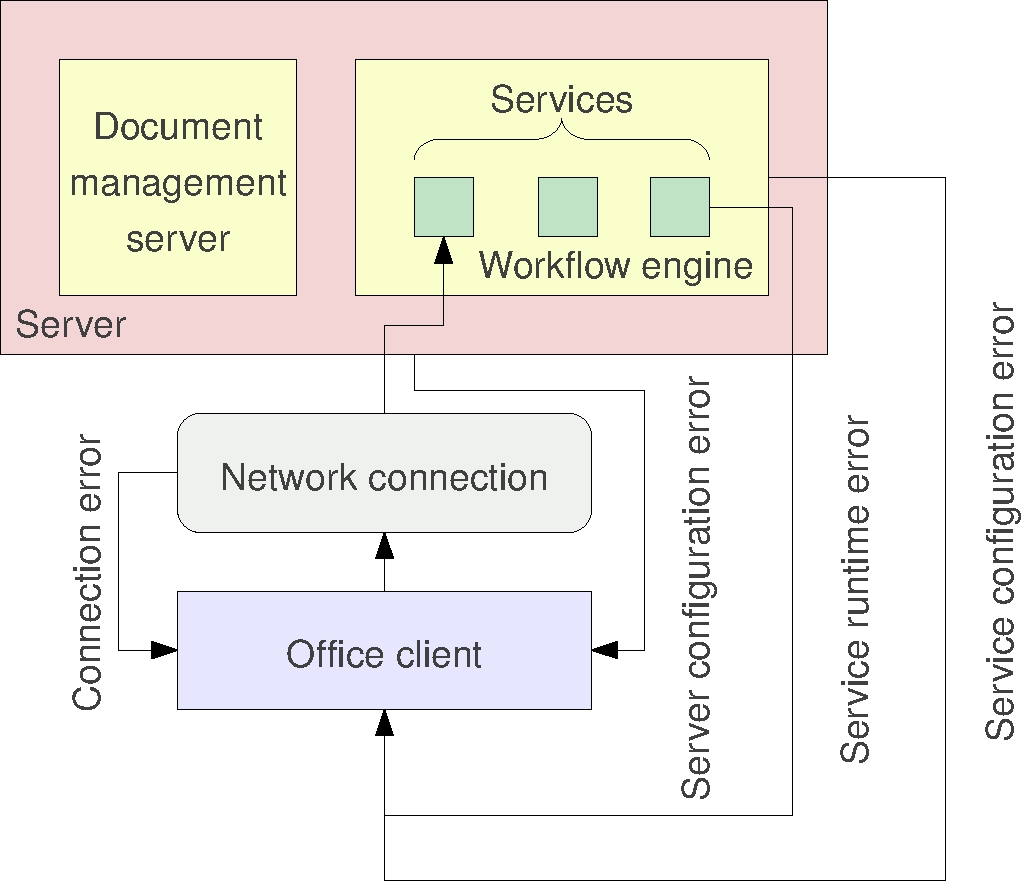
\includegraphics[width=300px,keepaspectratio]{error-levels.pdf}
\caption{Different levels of error handling in the extension}
\label{fig:error-levels}
\end{figure}

There are multiple levels where error handling should be implemented
(\autoref{fig:error-levels}):

\begin{itemize}
\item Accessing jBPM without a connection.
\item Accessing jBPM with a connection not configured for workflows.
\item Accessing a jBPM service which is not implemented by the server instance in question.
\item Handling errors from existing services.
\end{itemize}

\notocsubsubsection{Accessing without a connection}

Detecting this status is implemented in the BASIC macros:

\begin{itemize}
\item Macros call the \emph{getCurrentConnection()} function get the connection reference.
\item \emph{getCurrentConnection()} gets the current connection from the authentication manager (which is always available, since it is a singleton).
\item In case there is already a connection, it returns the reference. If there is no connection, it calls the \emph{getConnection()} function, that shows the connection dialog.
\end{itemize}

In case the user cancels the connection dialog, the action is cancelled, this
way the Java implementation can assume there is always a connection available.

\notocsubsubsection{Accessing without workflow support}

The user always has the possibility to leave the workflow URL of a server
configuration empty. In this case the extension does not try to connect,
either.

Later during workflow-related operations the control flow always starts with the following steps:

\begin{itemize}
\item get a reference to the current connection
\item call the \emph{getWFHandler()} method of the connection, to check if workflow support is available
\end{itemize}

In case the second step fails, the user gets an error message explaining the issue.

\notocsubsubsection{Checking workflow services}

The jBPM support listing available services, however that is more about serving as
a user guide to show what can be done, rather than a page to be machine-parsed.
The already mentioned TagSoup parser could be used to extract the necessary
information, but the page is not part of any stable API, so that approach could
easily break with the next jBPM version.

A better method is to properly handle all JSON parsing exceptions. This is
possible because in case a service is not supported, a HTML error is returned
by the server, which -- of course -- cannot be handled by the JSON parser.

Using this technique we can inform the user about exactly what required service
is missing on the server.

\notocsubsubsection{Errors in existing services}

A rather generic approach would be to check the HTTP code to detect errors, but it has two problems:

\begin{itemize}
\item The server returns HTTP 200 (\emph{OK}) even in case the HTML title of the page is \emph{HTTP 401}.
\item Even if the code would not be 200, we can't distinguish between service errors and non-existing services, unless different error codes are used (e.g. 500 for service errors, 503 for unavailable services).
\item One can also argue that HTTP error codes are to be used by the application server itself, not by servlets running on the server.
\end{itemize}

A better method is to check the content-type, and -- in case it is HTML -- the
title of the page.  If the content-type is unexpected, that will mean the
service is not available, as described above. Otherwise, the title of the
returned HTML page correctly contains the error code.

An example is when a login fails, in that case the \emph{HTTP 401} error code
is properly returned in the rendered HTML error page.
